\section{DFTB}

In this section results obtained by DFTB for ethylene carbonate (EC) with NaTFSI or LiTFSI salts are presented as well as for mixtures of EMIM-TFSI ionic liquid (IL) with different amounts of water. Two approaches are shown - the standard based on Slater-Koster parameters and extended Tight Binding (xTB) GFN2 variant proposed by Grimme et. al.~\cite{gfn-2}. For both of them, all simulations were performed in NVT ensemble with temperature $T = 298$~K.

\subsection{Ethylene carbonate with Na/Li TFSI salt}

\begin{figure}[ht]
    \centering
    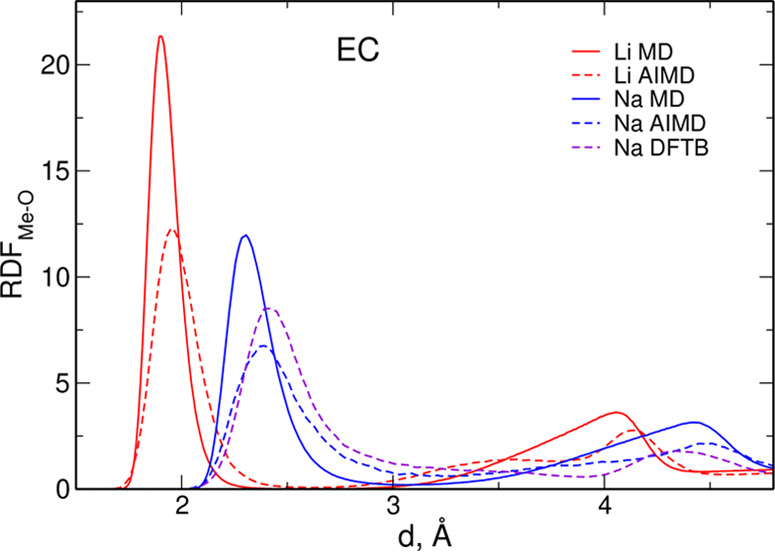
\includegraphics[width=0.4\textwidth]{img/5-alternatives-to-aimd/1-carbonates/rdf.png}
    \singlespacing
    \caption{Radial distribution functions for Me-O pairs for electrolytes based on EC obtained from classical MD, AIMD and DFTB MD simulations}
    \label{fig:dftb-carbonates-rdf}
\end{figure}

Results shown in this section were obtained to have comparison with AIMD results described in sections~\ref{section:carbonates-structural} and~\ref{section:carbonates-spectra}. Simulations were performed with the use of the DFTB+ v.~18.2 software~\cite{dftb-plus} with the 3ob-3-1 parameter set~\cite{3ob-1,3ob-2,3ob-3,3ob-4}. This set does not contain parameters for lithium, so only neat solvents and NaTFSI solution in EC were studied. The compositions of all systems were the same as for AIMD. These data were published in the article~\cite{carbonates}. In addition, systems studied by AIMD were simulated in DFTB+ v. 22.2 package in the xTB-GFN2 approach where it was possible to also include systems with lithium salt.

\begin{figure}[ht]
    \centering
    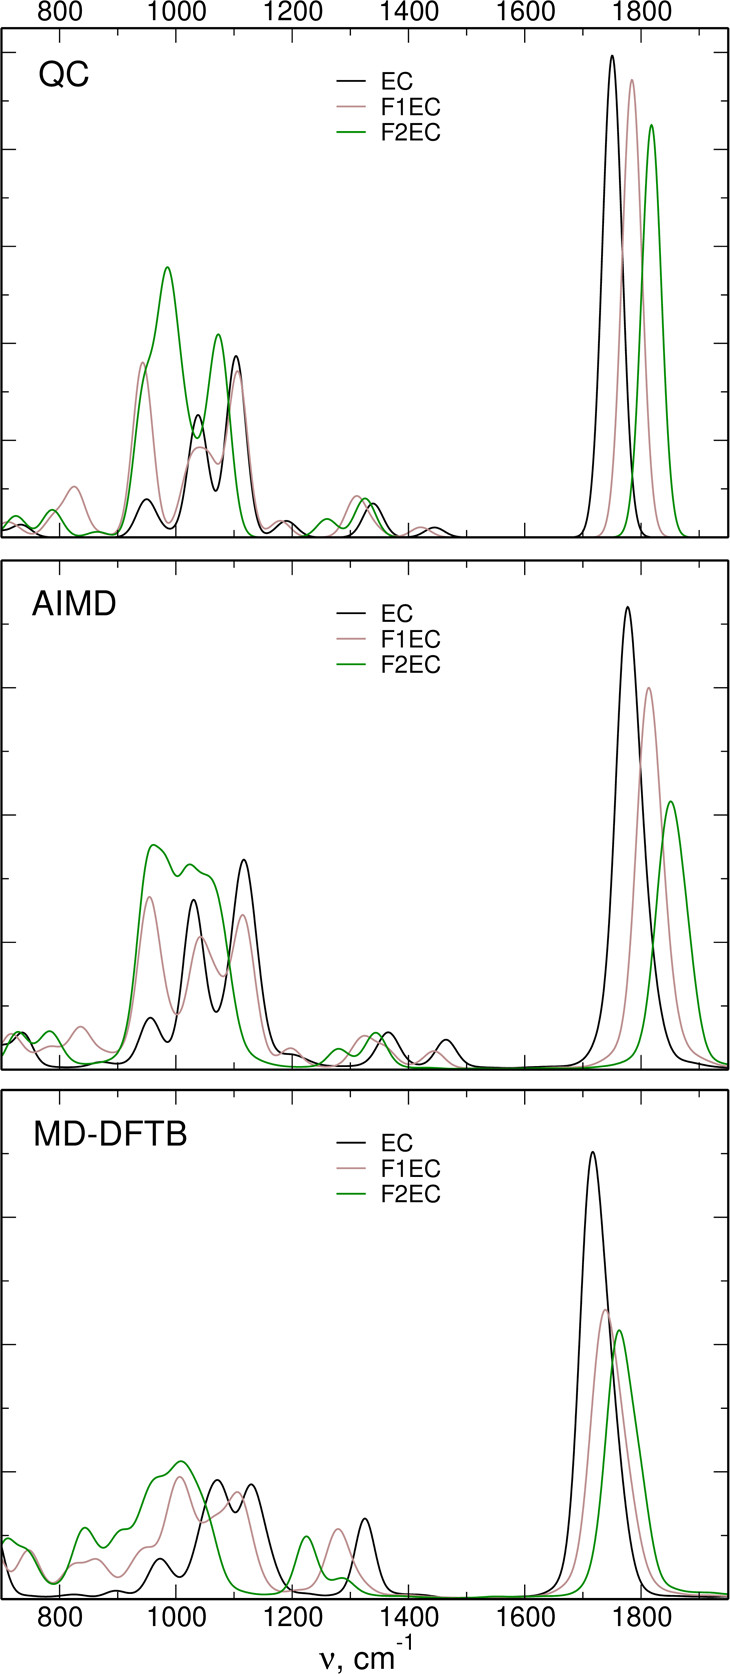
\includegraphics[width=0.4\textwidth]{img/5-alternatives-to-aimd/1-carbonates/ir-neat-solvents.png}
    \singlespacing
    \caption{Infrared spectra of neat solvents obtained from QC calculations or from AIMD and DFTB MD simulations}
    \label{fig:dftb-carbonates-ir-neat-solvents}
\end{figure}

Figure~\ref{fig:dftb-carbonates-rdf} presents RDFs for Me-O pairs obtained from different MD approaches. For Na-EC systems, the maximum in AIMD is located at higher distance that for classical MD (what was described previously). In DFTB it is shifted to distances longer than in AIMD (2.38~{\AA} vs 2.40~{\AA}) and the maximum is broader. Therefore it is expected that the interactions between sodium cation and EC are weaker in DFTB simulations than those in AIMD.

\begin{figure}[ht]
    \centering
    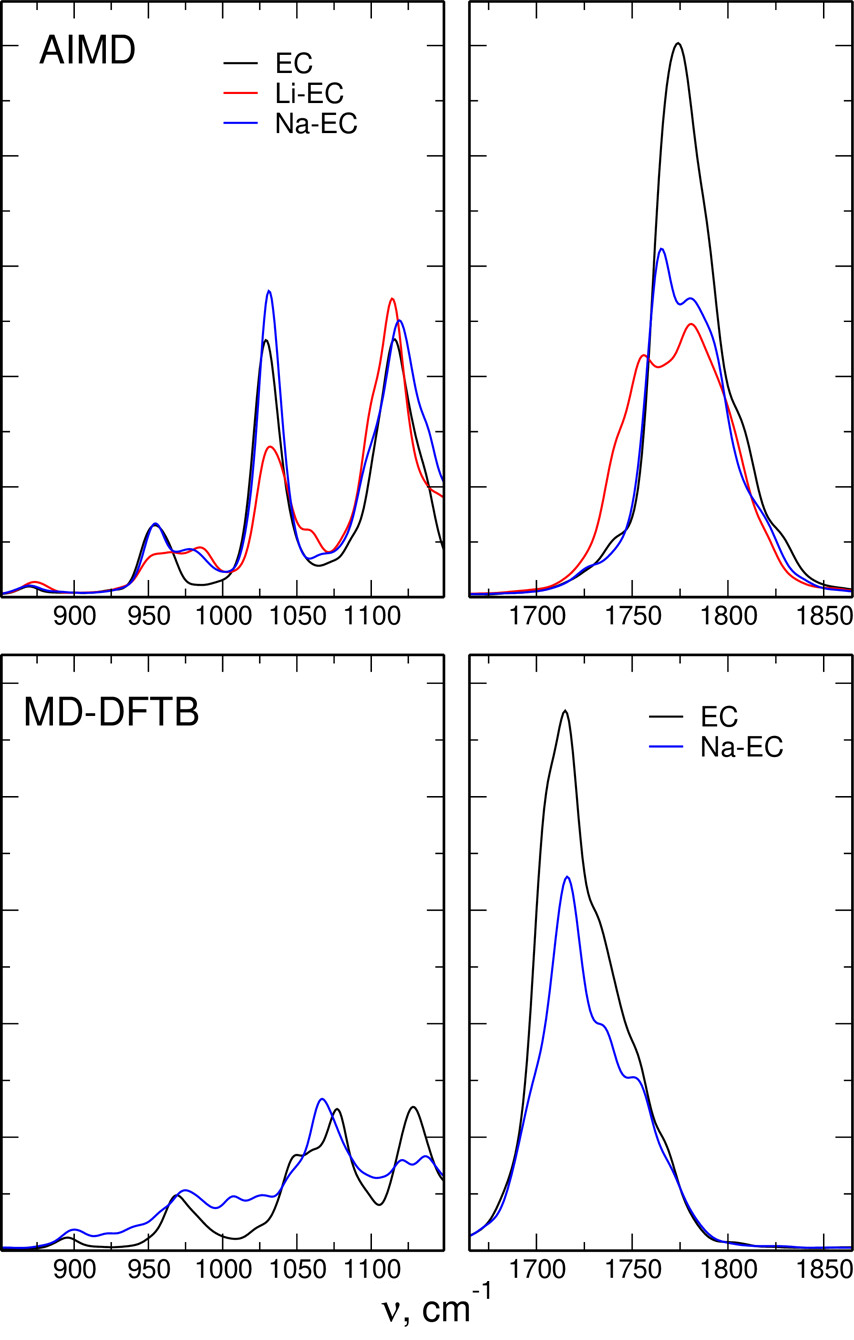
\includegraphics[width=0.4\textwidth]{img/5-alternatives-to-aimd/1-carbonates/ir-electrolytes.png}
    \caption{Infrared spectra of solvents and electrolyte solutions obtained from AIMD and DFTB MD simulations}
    \label{fig:dftb-carbonates-ir-electrolytes}
\end{figure}

Figure~\ref{fig:dftb-carbonates-ir-neat-solvents} presents IR spectra for neat solvents obtained from different approaches. For DFTB, as in AIMD or QC calculations, fluorination of the solvent shifts the C=O stretching band towards higher energies, from 1717~cm$^{-1}$ to 1739 and 1763~cm$^{-1}$. However, observed frequencies are lower than in AIMD and also differences between solvents are smaller. General features between 800 and 1200~cm$^{-1}$ in AIMD and DFTB are similar, there are some differences in the intensity pattern.

IR spectra for electrolyte solutions are presented in Figure~\ref{fig:dftb-carbonates-ir-electrolytes}. The main difference which could be observed is that, in opposition to AIMD, the position of C=O band between neat solvent and the electrolyte remains unaffected. However, small blue shifts of bands between 850-950~cm$^{-1}$ are observed as for the NaTFSI in EC in AIMD.

\begin{figure}[H]
    \centering
    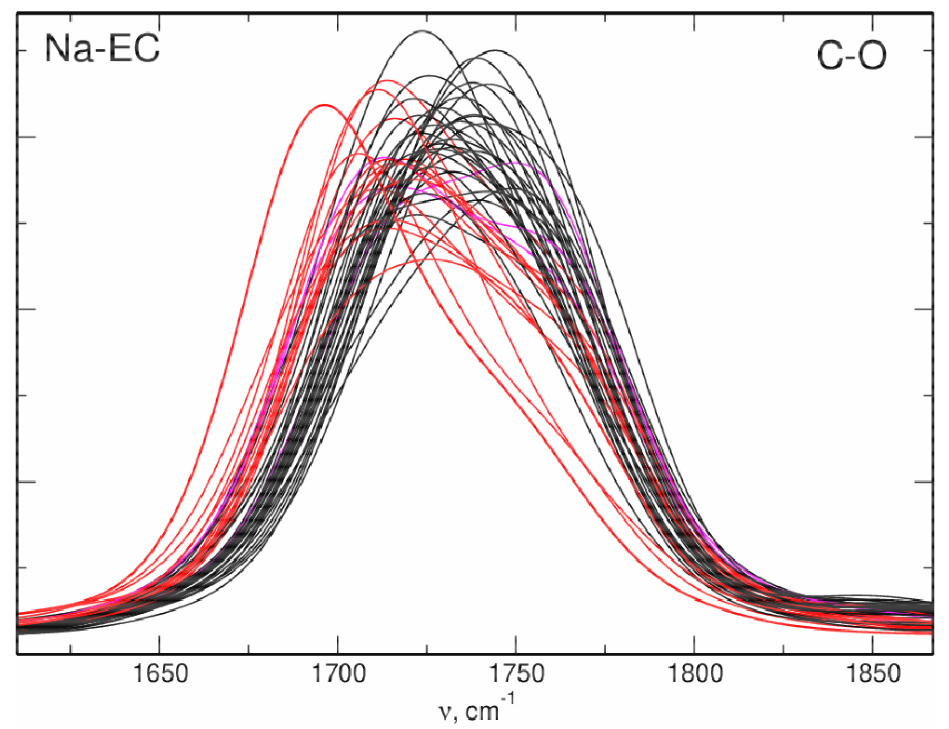
\includegraphics[width=0.4\textwidth]{img/5-alternatives-to-aimd/1-carbonates/ft-c-o.png}
    \singlespacing
    \caption{Fourier transforms of C-O distances in DFTB MD simulations. Free solvent molecules are marked in black, molecules interacting with Na$^{+}$ in red, and in magenta molecules interacting with cations for only a~part of the MD trajectory. Thick red line marks the molecule interacting with 2 Na$^{+}$ ions}
    \label{fig:dftb-carbonates-ft-c-o}
\end{figure}

Similarly as in AIMD simulations, FTs of C-O distances for Na-EC system were obtained and are shown in Figure~\ref{fig:dftb-carbonates-ft-c-o}. Different colors mark free and interacting with cation solvent molecules; additionally few molecules interacting with cation only for a~part of the simulation are marked. Again, interaction lowers the position of the maximum of the FT, and the effect is less visible for molecules which do not interact for the whole time of the simulation. In addition, the biggest shift is observed for the sole molecule which was interacting simultaneously with two Na$^{+}$ cations. However, differences between maximum positions are smaller than in the AIMD. This results does not agree with the IR spectrum obtained from DFTB simulation, as there the shift of C=O band position was not observed.

\begin{figure}[ht]
    \centering
    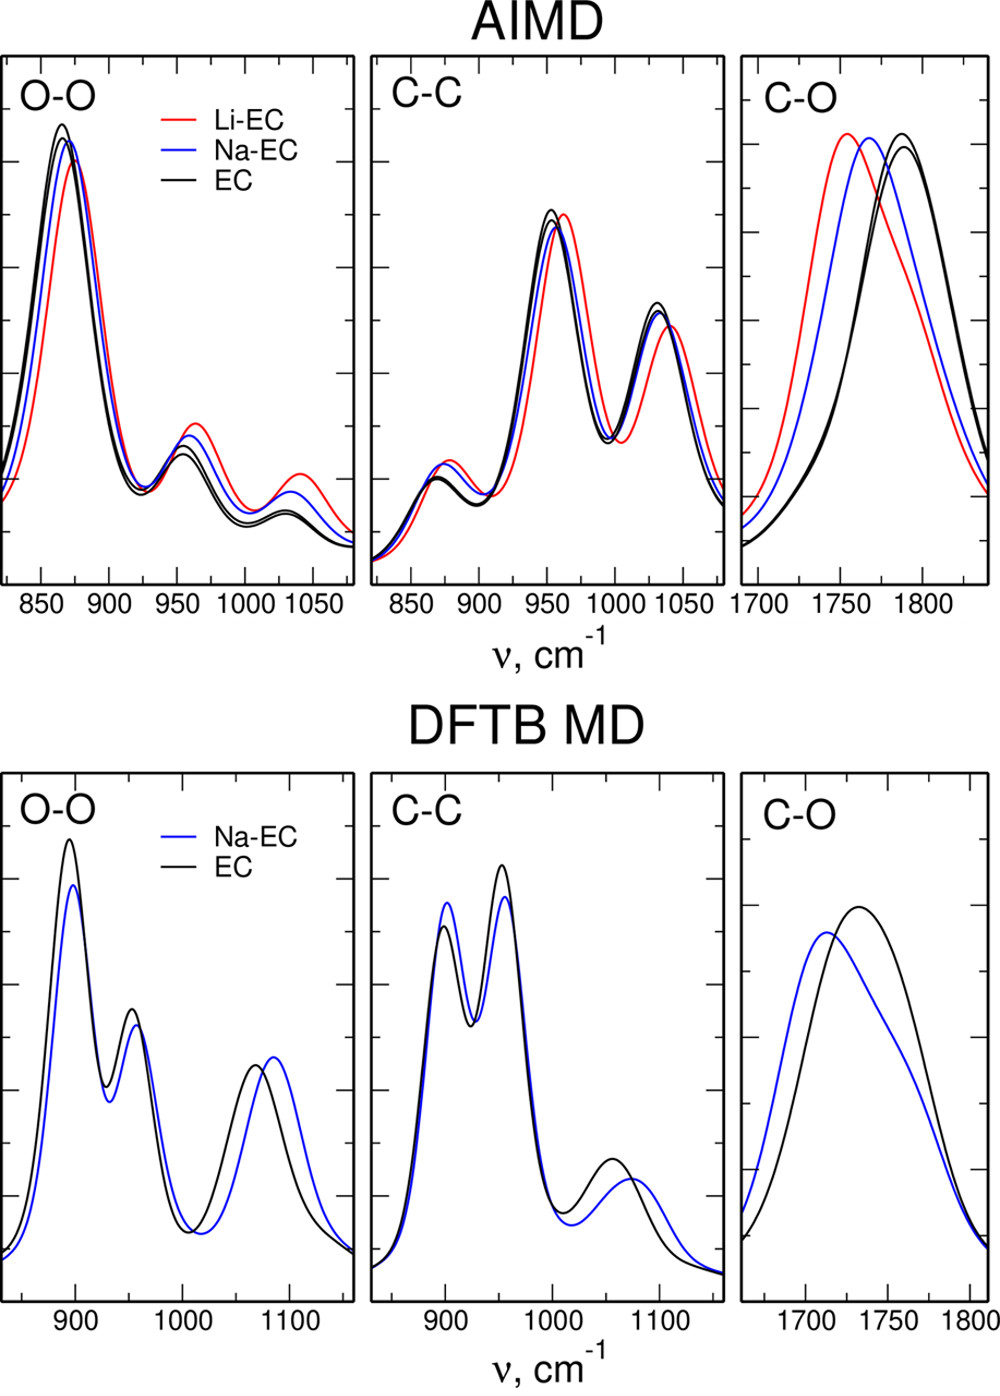
\includegraphics[width=0.4\textwidth]{img/5-alternatives-to-aimd/1-carbonates/ft-averages.png}
    \caption{Averaged Fourier transforms of interatomic distances in AIMD and DFTB MD}
    \label{fig:dftb-carbonates-ft-averages}
\end{figure}

In Figure~\ref{fig:dftb-carbonates-ft-averages} averaged FTs of interatomic distances are presented and compared with AIMD results. Here, in opposition to IR spectrum, the shift of the maximum for C=O bending is visible. It is unclear why such difference is observed. For DFTB simulations for every step of the trajectory, partial charges for each atom in the system are determined. The dipole moments are calculated based on these charges. Probably, used parametrization was not able to produce correct partial charges for sodium cation and the C~and O~atoms from the C=O group when they are affected by direct interaction.This led to almost unchanged positions of bands in the IR spectrum.

\begin{figure}[ht]
    \centering
    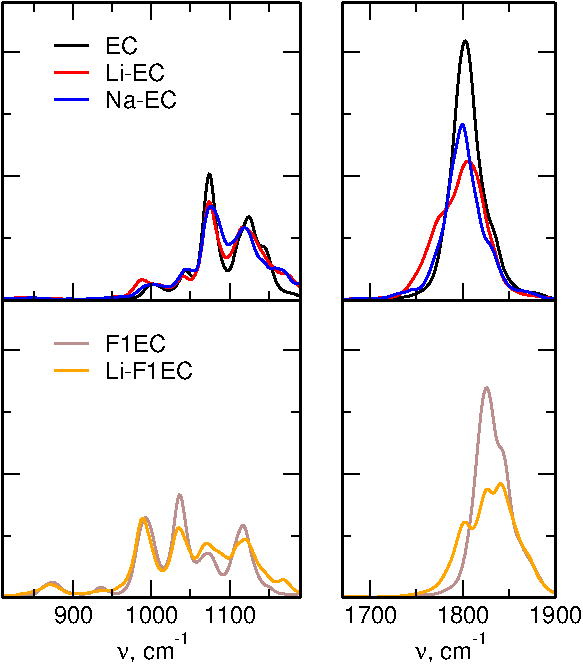
\includegraphics[width=0.4\textwidth]{img/5-alternatives-to-aimd/1-carbonates/xtb.png}
    \caption{Infrared spectra obtained from GFN2-xTB MD simulations}
    \label{fig:dftb-carbonates-xtb}
\end{figure}

Figure~\ref{fig:dftb-carbonates-xtb} presents IR spectra obtained in the GFN2-xTB approach. The effect of solvent-Me$^{+}$ interactions is visible for the C=O stretching band. In the spectrum of LiTFSI in EC a~shoulder appears on the low energy side of the main band, with the energy 29~cm$^{-1}$ lower than the maximum for neat~EC. There is also a~small red shift of 3~cm$^{-1}$ in the position of the maximum calculated for NaTFSI/EC electrolyte. The maximum in the LiTFSI solution in F1EC is red-shifted by 23~cm$^{-1}$ with respect to neat F1EC. The shift for NaTFSI electrolyte is much too small, but for LiTFSI the results are comparable to AIMD results. However, there is no blue-shift observed for the ring breathing mode. Perhaps the analysis of FTs of interatomic distances could reveal some frequency shifts not seen in the IR spectra.

In this case, DFTB simulations took shorter computational time than AIMD, however the results are worse than AIMD results with respect to experimental values. The main disadvantage of DFTB for studied systems is lack of Slater-Koster parameters for lithium and incorrect reproduction of the shift of C=O stretching band in the IR spectrum. It clearly shows the need of more appropriate parametrization, because the 3-ob-3-1 used here was mostly developed for biological systems, not electrolytes. GFN2-xTB approach is free from the limitation related to the parameters for lithium. It resulted in IR spectra more close to those obtained from AIMD than with 3-ob-3-1; the effect of red-shift of C=O band for lithium-based electrolytes was successfully reproduced. However, still results for sodium-based electrolytes are not satisfactory and the shift of the ring-breathing mode is not observed.

\cleardoublepage

\subsection{EMIM-TFSI with water}

In this section results obtained with different DFTB parametrizations as well as with xTB variants: GFN1 and GFN2 are presented. Simulations were performed in DFTB+ v.~22.1~\cite{dftb-plus}. For simulations of liquid water standard DFTB parametrizations were used: 3-ob-3-1~\cite{3ob-1,3ob-2,3ob-3,3ob-4}, matsci~\cite{matsci}, mio~\cite{mio}, ob2~\cite{ob2} and matsci variants improved to reproduce structural parameters of bulk waterk, named here as water-matsci and water-matsci-uff~\cite{water-matsci}. In addition, xTB variants: GFN1 and GFN2~\cite{xtb,gfn-2} were used for such simulations. Because from parametrizations mentioned, only 3-ob-3-1 covered all elements present in the IL, only this one was used for simulations for neat EMIM-TFSI and $x = 0.5$ system. From xTB variants, GFN2 resulted in more accurate results for bulk water, so this was the only method in this approach used for ILs. The length of the trajectory and other parameters of MD simulations were the same as for the AIMD simulations, the last 30~ps were used for analysis.

\begin{figure}[ht]
    \centering
    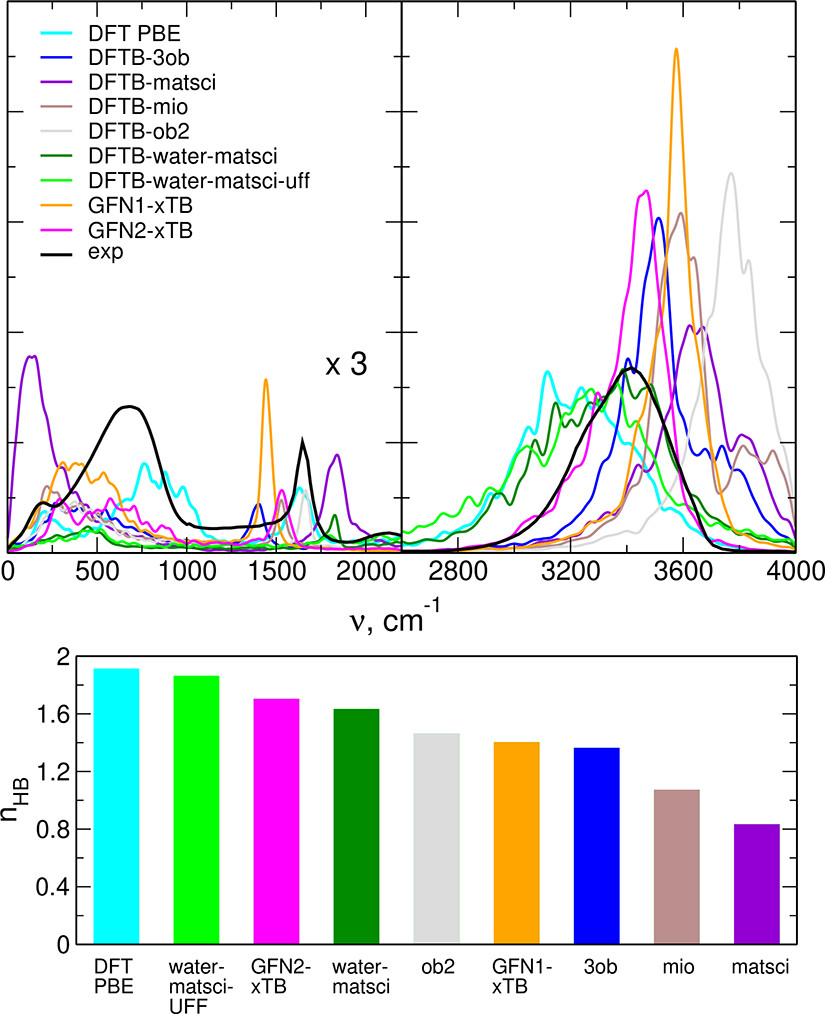
\includegraphics[width=0.45\textwidth]{img/5-alternatives-to-aimd/2-il-h2o/ir-hb.png}
    \caption{Infrared spectra calculated for bulk water in different DFTB parametrizations (top), average number of hydrogen bonds per water molecule (bottom)}
    \label{fig:dftb-il-h2o-ir-hb}
\end{figure}

Figure~\ref{fig:dftb-il-h2o-ir-hb} shows IR spectra of bulk water obtained in different parametrizations. The low-frequency region in every case is poorly reproduced. In the O-H region the best performing were water-matsci and water-matsci-uff parametrizations, specially designed for water. Next to these two were general parameter sets: GFN2, 3ob and GFN1. In the bottom part of Figure~\ref{fig:dftb-il-h2o-ir-hb} average numbers of HBs per water molecule are shown. The best in reproducing O-H region are the sets which predict the number of HBs close to the DFT data. However, there is no direct relation between average number of HBs to the quality of the spectrum, because 3ob which performs better than GFN1 and ob2 in reproduction of the spectrum, is worse at HBs number prediction.

\begin{figure}[ht]
    \centering
    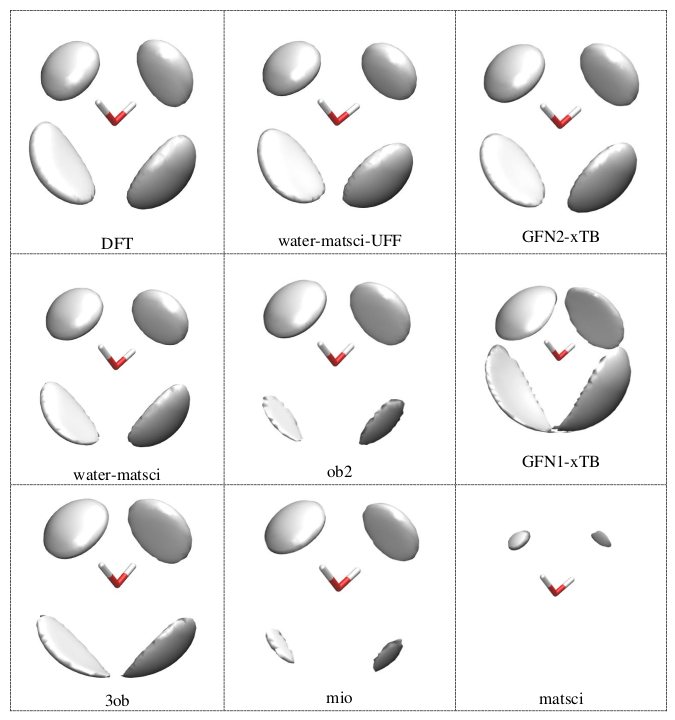
\includegraphics[width=0.45\textwidth]{img/5-alternatives-to-aimd/2-il-h2o/sdf-water.png}
    \caption{Spatial distribution functions of oxygen atoms around water molecules in bulk water obtained in DFTB simulations. Surfaces of particle density 100 atoms/nm$^3$ are shown}
    \label{fig:dftb-il-h2o-sdf-water}
\end{figure}

A~possible explanation of these differences come from SDFs presented in Figure~\ref{fig:dftb-il-h2o-sdf-water}. 3ob parametrization gives result closer to the tetrahedral structure of water than GFN1 and ob2. To summarize this part, the best performance was obtained for parameters developed specially for description of water: water-matsci and water-matsci-uff. From general parametrizations, GFN2 was well performing.

Spectra for IL and IL mixture with water are presented in Figure~\ref{fig:dftb-il-h2o-ir-dft-vs-dftb}. The 3ob patametrization for both cases predicts two main IR bands in the range of 1000-1300~cm$^{-1}$ instead of three present in DFT results. GFN2 correctly reproduces number of bands, and their frequencies are closer to DFT results. Next, in the region above 3000~cm$^{-1}$ in neat IL, results are similar and again GFN2 gives frequencies closer to DFT values. Significant differences are observed in the system with $x = 0.5$. In both cases an intense band at 3500~cm$^{-1}$ appears; in 3ob results there is also an increased IR intensity above 3700~cm$^{-1}$.

To explain this effect, trends in HB formation were studied. In Figure~\ref{fig:dftb-il-h2o-sdf-il} SDFs for ILs simulated in GFN2 are presented. When compared to SDFs for DFT results in Figure~\ref{fig:il-h2o-sdf} it is visible that in this case TFSI$^{-}$ and water oxygen atoms are more evenly distributed around EMIM$^{+}$ cations and the probability is concentrated not only close to the H$_{Im}$ hydrogen atoms, but also near methyl groups.

Average numbers of the most abundant types of HBs are plotted in Figure~\ref{fig:dftb-il-h2o-hb-averages}. In the 3ob results, average numbers of all main types are reduced compared to DFT, so in this method the HB formation ability is smaller. It may explain the maximum at about 3800~cm$^{-1}$ in the IR spectrum, as this could be related to bigger number of "free" O-H bonds of water molecules in the system, contributing to this part of the spectrum. For GFN2, as it was expected from SDFs, there are more HBs involving methyl group hydrogen atoms. In HBs with water as a~donor, the ratio of anion or water acceptors is changed in favor of the anions. Nevertheless, it is not clear why for both DFTB approaches the band at 3500~cm$^{-1}$ develops.

\begin{figure}[H]
    \centering
    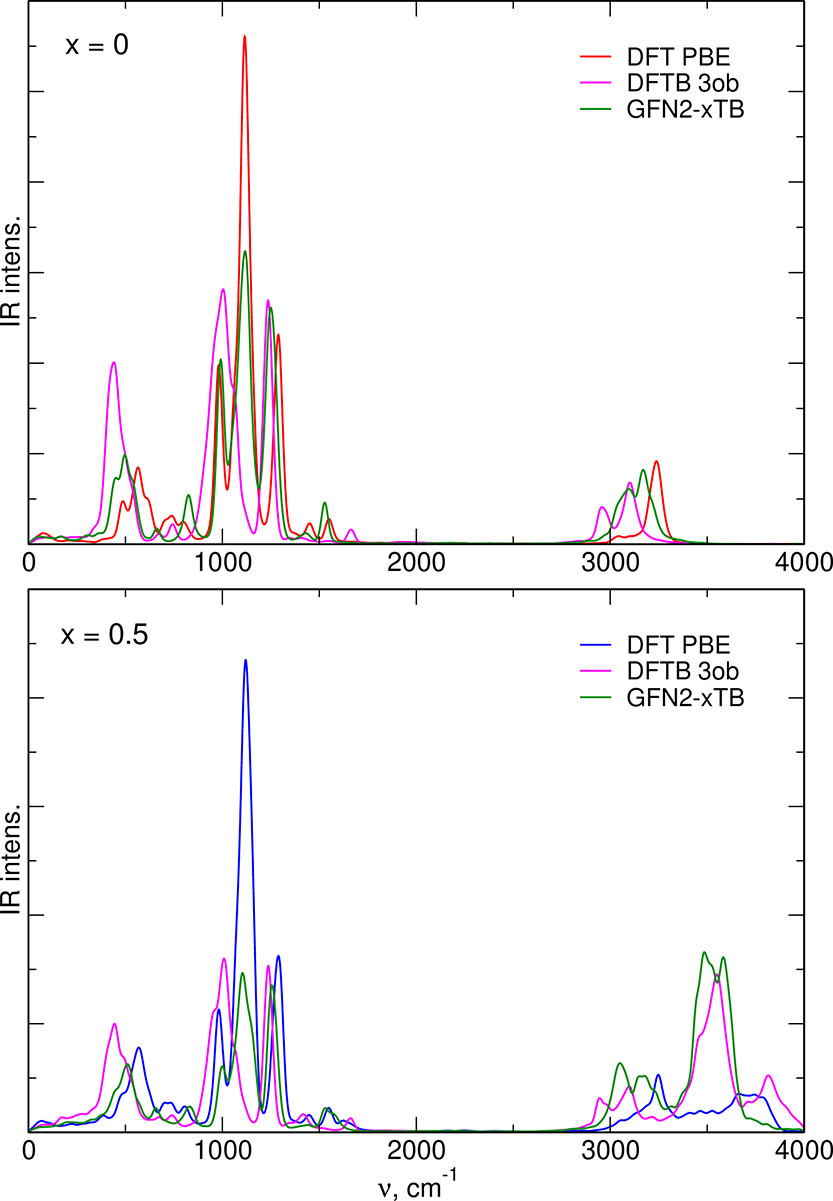
\includegraphics[width=0.45\textwidth]{img/5-alternatives-to-aimd/2-il-h2o/ir-dft-vs-dftb.png}
    \singlespacing
    \caption{Infrared spectra of neat IL and the mixture with water obtained from MD based on PBE DFT or two DFTB parametrizations}
    \label{fig:dftb-il-h2o-ir-dft-vs-dftb}
\end{figure}

\begin{figure}[H]
    \centering
    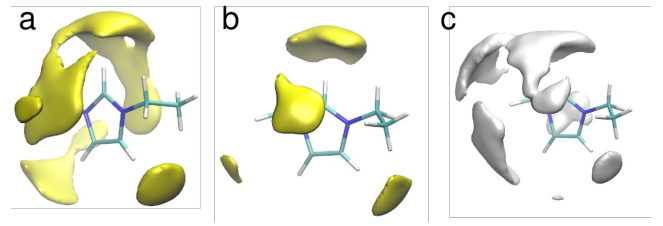
\includegraphics[width=0.4\textwidth]{img/5-alternatives-to-aimd/2-il-h2o/sdf-il.png}
    \singlespacing
    \caption{Spatial distribution functions of oxygen atoms around EMIM$^{+}$ cations in simulations from GFN2-xTB method: (a) TFSI$^{-}$ anions in the neat IL, (b) TFSI$^{-}$ anions in the $x = 0.5$ mixture, (c) water molecules in the $x = 0.5$ mixture. Surfaces of particle density 10 atoms/nm$^3$ are shown}
    \label{fig:dftb-il-h2o-sdf-il}
\end{figure}

To summarize, for water in DFTB the specially developed parametrizations water-matsci and water-matsci-uff were the best performing, as well as the general-purpose GFN2 method. However, for IL mixtures with water neither of used parametrizations was able to correctly reproduce changes in IR spectrum caused by presence of water due to their improper description of IL-water hydrogen bonding. Therefore, for this purpose DFTB parametrizations need further corrections.

\begin{figure}[ht]
    \centering
    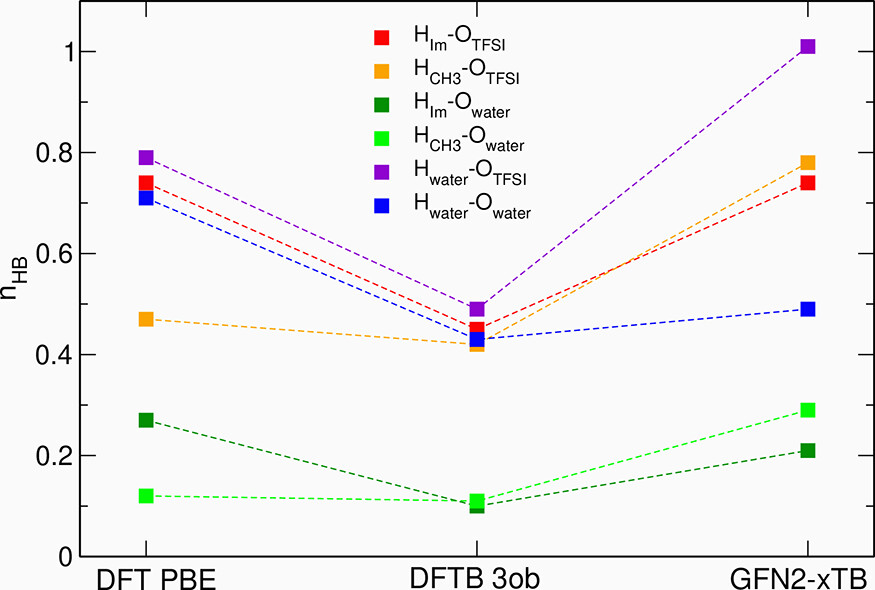
\includegraphics[width=0.4\textwidth]{img/5-alternatives-to-aimd/2-il-h2o/hb-averages.png}
    \caption{Average numbers of the most abundant hydrogen bonds obtained for $x = 0.5$ from MD simulations based on DFT or DFTB. Lines are only to guide the eye}
    \label{fig:dftb-il-h2o-hb-averages}
\end{figure}

For described in this section systems, DFTB method was able to reproduce in most cases approximately the positions of bands in IR spectra. However, observed shifts were strongly dependent on the used parametrisation. From the general-purpose methods both for carbonate-based electrolytes as well as for EMIM-TFSI mixtures with water, GFN2-xTB was the best performing. For bulk water, there was a~specially developed parametrisatio for this purpose, and this one resulted in the closest spectrum to this obtained from AIMD. Although, still GFN2-xTB method was not able to correctly reproduce all changes observed in AIMD spectra. Thus, DFTB seems as a~promising alternative to AIMD due to its reduced computational cost, however it still needs improved parametrizations to be reasonable for use in analysis of vibrational spectra.

\cleardoublepage